\section{Background}
This section outlines the definitions of boolean circuits and indistinguishability obfuscation that are essential to this paper.
\par
\subsection{Boolean Circuits}
Real world programs are compiled into a sequence of machine instructions that can be interpreted by a processing unit (CPU) manipulating a finite number of $bits$ at a time. The CPU is a chip that is made of logical gates that are made of a few transistors. In this context, boolean circuits are a powerful model that can express any algorithm we can run on a CPU\cite{cpu}.
\par
Complexity Theory defines a \textit{Boolean Circuit} $C$ with $n$ inputs and $m$ outputs as a finite, labelled, directed acyclic graph. It contains $n$ nodes with no incoming edges or ancestors; called the input nodes and $m$ nodes with no outgoing edges or successors, called the output nodes. All other nodes are called gates and represent the logic operation AND, OR and NOT\cite{bool}. Simply put, a \textit{Boolean Circuit}  is a diagram showing a combination of logic operators to a drive an output from an input. By associating a boolean function with each gate, a boolean circuit computes an arbitrary function $f \in F :  \{0,1\}^n \to \{0,1\}^m$. Two common properties are associated with boolean circuits: 
\begin{enumerate}  
	\item The $size$ of a circuit is the number of non-input vertices that it contains. 
	\item The $depth$ of a circuit is the length of the longest directed path from an input vertex to an output vertex. 
\end{enumerate}
Because of the acyclic and oriented nature of the circuit, each node can be represented as receiving its inputs from a lower order depth only. To evaluate a circuit, we process the nodes in an increasing order of depth by applying the associated boolean operation on the input vertices. The result is passed to the higher order nodes.
\par
\begin{figure}[h]
	\center
	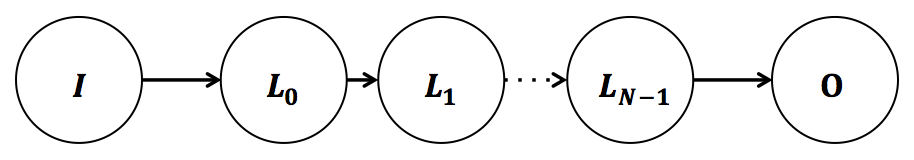
\includegraphics[width=0.8\textwidth]{img/graph.png}
	\caption{Simple high level representation of a boolean circuit}
\end{figure}
\par
Size and Depth give an indication of the computation necessary to evaluate a circuit. Size is a rough measure of the computation time a single processor would need for a sequential circuit evaluation. Depth is an important cost metric for time efficiency in a parallel execution environment where the size is no longer the main bottleneck\cite{notes}. 
\par 
Another  established circuit property that is relevant to our study is the $width$ of a circuit\cite{clark}. If the circuit is arranged in levels such that the input of each level are connected from lower order levels exclusively, we define the width $w$ as the maximum number of gates contained in single level.
\par
The formal study of circuit complexity is beyond the scope of this paper. We should however quickly mention the notion of \textit{Circuit Family}. Our definition limits the size of input to a fixed number of bits. The notion of boolean circuit $C_n$ computing $f_n$  is generalised to a family of circuits C which is a collection of boolean circuits $\{C_1, C_2, C_3, \cdots\}$ such that there is one circuit $C_i$ that computes F on i inputs.
%-----------------------------------------------------------
%
%
%-----------------------------------------------------------
\subsection{Indistinguishability Obfuscation}
Obfuscation must meet two requirements, as defined by Barak et al.\cite{barak}:
\begin{enumerate}
	\item The functionality of the obfuscated programme must remain identical to the functionality of the original, un-obfuscated programme.
	\item Anything (and everything) that can be efficiently computed from Oc can be efficiently computed given oracle access to C. i.e. Oc does not disclose any information about the input other than what C does. 
\end{enumerate}
The first requirement is trivial and means that for any input programme $C$, an Obfuscator $O$ produces a new programme $O_C$ where the functionality of $O_C$  is identical to the functionality of $C$. This condition means that given an input space $I$ we have $ \forall x \in I, C(x) = O_C(x)$.
\par
The second requirement is less trivial and also known as the Virtual Black Box $(VBB)$ requirement. It implies that there is no ``leakage`` of information, other than the input and the output. This means that it is impossible to tell whether an output was produced from the computation of $C$, or from the computation of $O_C$. An adversary can learn a predicate of $O_C(x)$ with the same probability of learning it from $C(x)$. 
\par
Barak et al. concluded that the VBB requirement is impossible to attain in certain situations\cite{barak}, however, it is possible to come close to meeting the second requirement, which in practice is enough to maintain the usefulness of obfuscation as an effective security measure. This is done by modifying the requirement of VBB, and replacing it with two weaker definitions that can still result in rendering a programme unintelligible in a meaningful and practical way. These definitions are namely indistinguishability $iO$ and differing-input obfuscation $diO$, which require that for any circuit pair $C_1$ and $C_2$ from the same circuit family $C$ that compute the same functionality $f$, the obfuscated versions of $C_1$ and $C_2$; $iO(C_1)$ and $iO(C_2)$ are perfectly indistinguishable. The probability of an observer being able to tell if an output was generated from $iO(C_1)$ or from $iO(C_2)$ is negligible.
\par
Some work has been done within the scientific community to develop real-life obfuscations that meet the requirements given by Barak et al. Garg et al.\cite{garg} published an obfuscation construction valid for all polynomial-size, log-depth circuits constructed under novel algebraic hardness assumptions. Based on this work, Banescu et al.\cite{tum} published a proof-of-concept implementation of this $iO$ construction.
However, to date there is no efficient practical implementation of Barak et al.\cite{barak} indistinguishability obfuscation requirement. The study of the security of functional obfuscators is beyond the scope of this paper.
\par
But this lack of ready-made obfuscators does not limit the ability of this paper to prove or disprove the hypothesis that obfuscation is ultimately limited by the hardware restraints of the operating system, as a simulation of an obfuscation-like process is sufficient for this purpose.

